\section{Zadanie 6}
\subsection{Opis problemu}
Celem tego zadania było znalezienie miejsc zerowych funkcji $ f_1(x) = e^{1 - x} - 1 $ oraz $ f_2(x) = xe^{-x} $ za pomocą wcześniej zaimplementowanych metod przy dokładności $ \delta = 10^{-5}$, $\epsilon = 10^{-5}$. Dobrać odpowiednio przedział i przybliżenie początkowe.
\subsection{Rozwiązanie}

Na samym początku, dla ułatwienia zadania, za pomocą biblioteki matplotlib wygenerowałem wykresy funkcji $ f_1(x)$ oraz $f_2(x)$.

\begin{figure}[!htbp]
  \centering  
  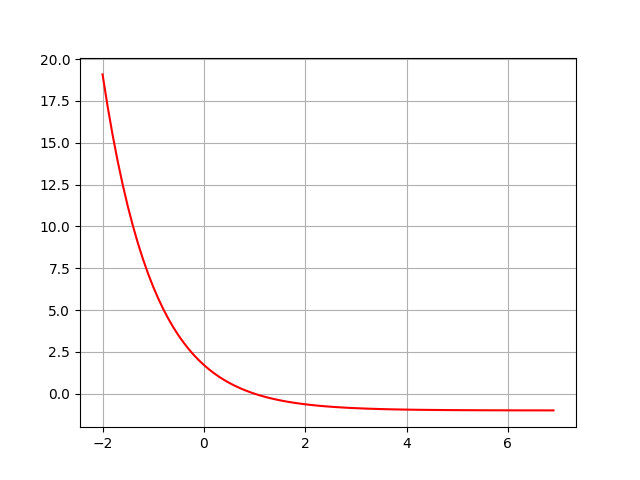
\includegraphics[totalheight=6cm]{../plots/ex6_f_1.png}
  \caption{Wykres $f_1(x) = e^{1 - x} - 1$}
\end{figure}

Z analizy wykresu (Rysunek 2) zaobserwowałem, że poszukiwane miejsce zerowe znajduje się w przedziale $ x \in [0.0, 2.0] $, ponadto

\begin{figure}[!htbp]
  \centering  
  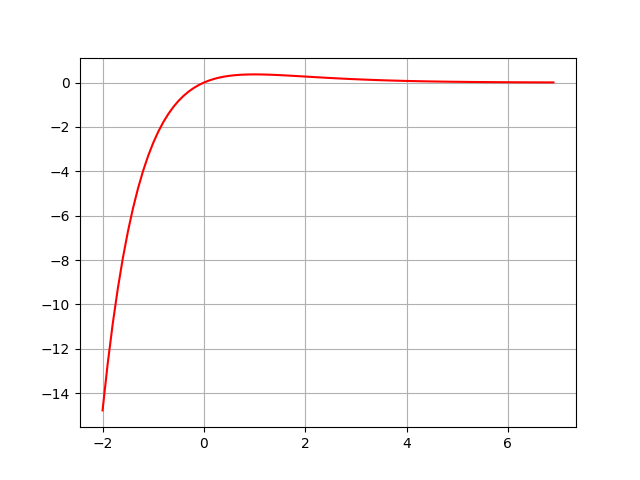
\includegraphics[totalheight=6cm]{../plots/ex6_f_2.png}
  \caption{Wykres $f_2(x) = xe^{-x}$}
\end{figure}


Z obserwacji wykresów wywnioskowałem, że dla pierwszej 

\subsection{Wynik}
Wyniki zestawiłem w tabeli poniżej: \\
\begin{center}
\begin{tabular}{|c|c|c|c|c|}
  \hline 
    Przedział & $x$ & $ f(x)$ & $i$ & $err$ \\
  \hline
  $ (0.0, 1.0) $ & 0.619140625 & 9.066320343276146e-5 & 9 & 0\\
  \hline 
  $ (0.1, 2.0) $ & 1.5120849609375 & 7.618578602741621e-5 & 13 & 0\\
  \hline
\end{tabular} 
\end{center}
